\documentclass[11pt]{article}

% Packages
\usepackage{graphicx}   % for pictures
\usepackage{amsthm}     % for math
\usepackage{amsmath}    %   more math
\usepackage{amsfonts}   %   more math
\usepackage{physics}    % more symbols
\usepackage{circuitikz} % for circuit diagrams
\usepackage{amssymb}    % math symbols
\usepackage{siunitx}    % units
\usepackage{mathrsfs}   % fancy text
\usepackage{color}      % colored letters for notes and reminders
\usepackage{float}      % for image location

%The amsthm package lets you format different types of mathematical ideas nicely. You use it by defining "\newtheorem"s as below:
\newtheorem{problem}{Problem}
\newtheorem{theorem}{Theorem}
\newtheorem*{proposition}{Proposition}
\newtheorem{lemma}[theorem]{Lemma}
\newtheorem{corollary}[theorem]{Corollary}
\theoremstyle{definition}
\newtheorem{defn}[theorem]{Definition}

% Magins

\setlength{\voffset}{0.1in}
\setlength{\paperwidth}{8.5in}
\setlength{\paperheight}{11in}
\setlength{\headheight}{14pt}
\setlength{\headsep}{0.5in}
\setlength{\textheight}{11in}
\setlength{\textheight}{8in}
\setlength{\topmargin}{-0.25in}
\setlength{\textwidth}{7in}
\setlength{\topskip}{0in}
\setlength{\oddsidemargin}{-0.25in}
\setlength{\evensidemargin}{-0.25in}

% For images in this document:
\graphicspath{ {images/} }

% User Defined Commands
\newcommand{\nder}[2]{\frac{d^{#1} #2}{d t^{#1}}}   % The nth derivative wrt t: {n}{x(t)}
\newcommand{\der}[1]{\frac{d #1}{d t}}              % Derivative wrt t: {x(t)}
\newcommand{\infint}{\int_{-\infty}^{\infty}}       % Integral from - infinity to + infinity
\newcommand{\infsum}[1]{\sum_{#1 = -\infty}^{\infty}}% Sum of a variable from - to + infinity
\newcommand{\para}[1]{\left( #1 \right)}            % Instead of writing parenthesis all the time



% Heading:
\usepackage{fancyhdr}
\pagestyle{fancy}
\lhead{Nicholas Pham}
\chead{ES 155}          %   Change the Class!!
\rhead{Homework 1}   %   Change the Problem Set Number!!


% ----- BEGIN DOCUMENT-----
\begin{document}

\textbf{\huge{ES 155 Homework 1}}    %   Change the Class and Problem Set Number!!
\normalsize

\begin{enumerate}
    \item % Problem 1
    Human balance can be thought of as a control system.  Though visual cues are very important, balancing with your eyes closed could be described by the system shown in Figure \ref{fig:humanbalance}:
    
    \begin{figure}[h]
        \centering
        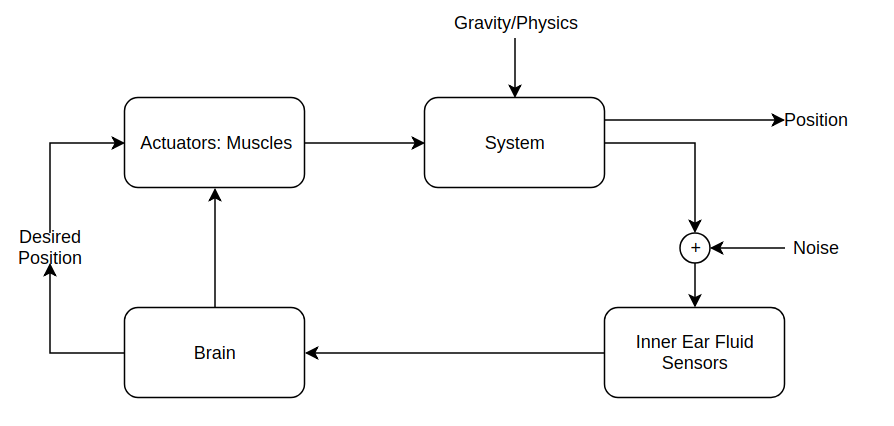
\includegraphics[width = 0.8 \textwidth]{ES155P1_1_balancediagram.png}
        \caption{Non-Visual Human Balance System Diagram}
        \label{fig:humanbalance}
    \end{figure}
    
    In this feedback control system, your brain decides on a desired body position, such as standing up straight.  It tells the muscles to move to such a position.  This force from the muscles and gravity are the inputs to the system, which outputs your body position.  Your inner ears contain some fluid which is used as a sensor, sensing some angular and linear position information, along with some noise, that is sent to the brain.  The brain then decides on some corrective action to keep you upright, and sends this to the muscles to continue the feedback loop.  Of course, all of these connections have some noise and other non-idealities which are not depicted in this diagram.
    
    \item % Problem 2
    Feedback systems occur everywhere in everyday life in addition to balancing on one leg.
    \begin{itemize}
        \item A thermostat is a classic example.  The sensing mechanism is a temperature sensor; on traditional thermostats is a metallic spiral with two different metals.  The two metals expand when heated at different rates, so the spiral contracts or expands as well.  This is used to turn on and off a switch, the actuating mechanism.  In this case, the control law is very simple: when the temperature is high enough that the spiral breaks the switch, the heating element is turned off.  When the temperature gets low enough the the spiral closed the switch again, the heating element is turned back on.  This is a simple on-off feedback system which attempts to provide robustness against changes in room temperature.  While the heating system is off, the room gradually cools down due to diffusion.  Without the system, it would continue to cool until the temperature reached equilibrium, typically with the outdoor temperature.  However, with the feedback loop, the heater is turned on when the temperature gets too low, so the heat will rise enough to remain in the desired temperature range.
        
        \item A more human example of a feedback system would be a bouncer at a party.  Given parameters such as the size of the room or the volume of the music, there is some optimal number or range of numbers of people to be at a party.  If there are too few, then the party might be boring and no one will want to be there.  But if there are too many people, this might encourage even more people to come until there could be a safety hazard.  In this system, the sensing mechanism is the bouncer.  He can look into the party and decide if it looks crowded or empty.  He can also use some counter to get an estimate of the crowd's size by keeping track of how many people have entered and exited.  His actuation mechanism for controlling the crowd size is choosing whether or not to let people into the party.  The control law would tell him to keep people waiting if the party was getting too large, or to allow people in if the party was small.  This system provides robustness against fluctuations in room occupancy.  However, there are some issues with this system.  While there is an easy mechanism for preventing party growth when there is a high demand, there is no way to quickly reduce party size.  In addition, the bouncer has no way to entice people to enter if there is no one waiting.
        
        \item A third example of a feedback system is a dynamic range compressor for audio.  These signal processors attempt to keep a continuous output level despite changes in input amplitude.  While some designs use a feed-forward method, many older designs use a feedback topology.  In these systems, the sensing mechanism is some amplitude detection circuit, which outputs a signal proportional to the signal amplitude at the output of the amplifier.  The actuation mechanism is some voltage controlled amplifier or similar device which can change its gain according to a control signal.  The control law enforces a negative feedback system: if the output level is high, then the controller turns the gain of the amplifier down.  Conversely, if the output amplitude is low, the controller turns the gain of the amplifier up.  In this way, this feedback system provides robustness in changing input amplitudes.  This type of dynamic range compression can be useful for recordings when a performer plays with inconsistent volume.
    \end{itemize}
    
    \item % Problem 3
    
    \item % Problem 4
    
    For the cruise-control system with dynamics
    
    \begin{align*}
        m\dot{v} = -av + u + \omega
    \end{align*}
    
    with the disturbance force $\omega$ ignored might have an open-loop control strategy to achieve $v_{ref}$:
    
    \begin{align*}
        u = \hat{a}v_ref
    \end{align*}
    
    where $\hat{a}$ is your estimate of $a$.
    
    \begin{enumerate}
        \item % Part a 
        The equilibrium point for this system occurs when there is constant velocity, or
        
        \begin{align*}
            m\dot{v} &= 0
        \end{align*}
        
        For the open-loop strategy above, this means that
        
        \begin{align*}
            m\dot{v} &= -av + u\\
            0 &= -av + \hat{a}v_{ref}
        \end{align*}
        
        Thus, the equilibrium point is 
        
        \begin{align*}
            \frac{\hat{a}}{a} &= \frac{v}{v_{ref}}
        \end{align*}
        
        In terms of $\beta = a/\hat{a}$,
         
        \begin{align*}
            \frac{v}{v_{ref}} &= \frac{1}{\beta}
        \end{align*}
        
        For the feedback law
        
        \begin{align*}
        u = -k_p(v - v_{ref})
        \end{align*}
        
        with $k_p = 10\hat{a}$, the equilibrium point is now
        
        \begin{align*}
            m\dot{v} &= -av + u\\
            0 &= -av - 10\hat{a}(v - v_{ref})\\
            \frac{v}{v_{ref}} &= \frac{10\hat{a}}{a + 10\hat{a}} \\
            \frac{v}{v_{ref}} &= \frac{1}{\frac{\beta}{10} + 1} = \frac{10}{\beta + 10}
        \end{align*}
        
        Figure \ref{fig:steadystates} shows the comparison between the feed-forward and feedback system topologies.
        
        \begin{figure}[h]
            \centering
            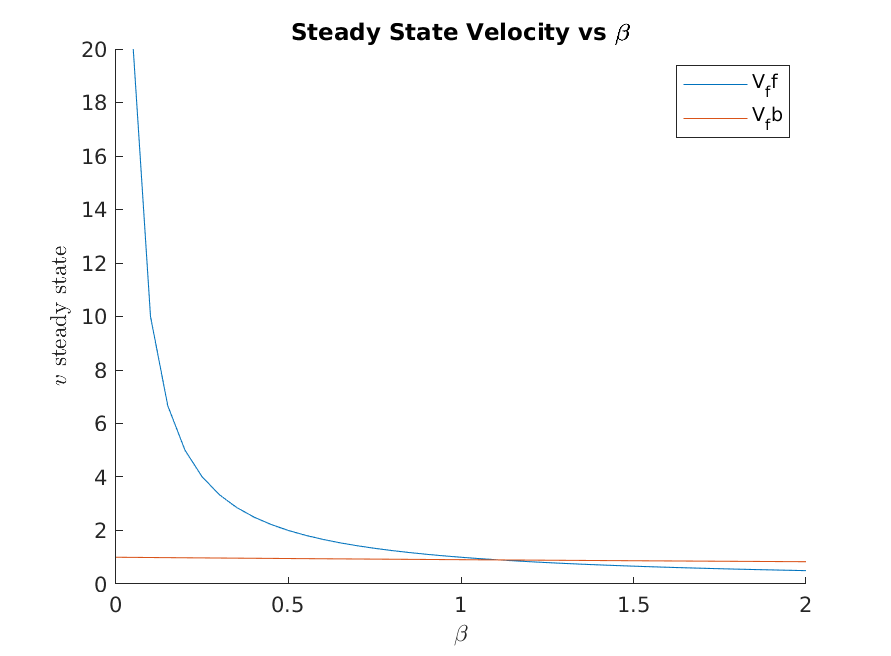
\includegraphics[width = 0.8 \textwidth]{ES155P1_4a_steadystatevsbeta.png}
            \caption{Steady State Velocity vs $\beta = a/\hat{a}$ for feed-forward and feedback systems}
            \label{fig:steadystates}
        \end{figure}

        As can be seen, the feedforward response is highly dependent on the accuracy of $\hat{a}$.  When $\hat{a} = a$, the velocity is exactly $v_{ref}$, but as the measurement error grows, the output velocity can be wildly different than the target.  On the other hand, we can see that the feedback system produces much more accurate velocity, even when the actual value of $a$ is twice that of the estimated value.
        
        \item % Part b
        To improve the feedback mechanism, a proportional-integral (PI) control law such as 

        \begin{align*}
            u = -k_p (v - v_{ref}) - k_i \int_0^t (v - v_{ref})dt
        \end{align*}

         could be used.  In this case, the steady state can be described by

        \begin{align*}
            m\dot{v} &= -av + u\\
            0 &= -av  - k_p (v - v_{ref}) - k_i \int_0^t (v - v_{ref})dt \\
            \text{Let } q=  \int_0^t (v - v_{ref})dt, &\qquad \dot{q} = v - v_{ref} \\
            0 &= -av -k_p \dot{q} - k_i q \\
            &= - a \left(\dot{q}+ v_{ref} \right) - k_p \dot{q} - k_i q \\
            \dot{q} &= -\frac{a}{a + k_p} v_{ref} - \frac{k_i}{a + k_p} q = v - v_{ref}
         \end{align*}

         For a PI controller, the integral controller is used to eliminate steady state error, which improves on the proportional gain case above.  In the proportional-only controller, there is always a finite error as long as the system does not have infinite gain.  However, by adding a negative component of the integration of the error, long-term offsets can be eliminated.

        \item % Part c
        
        
    \end{enumerate}

\end{enumerate}
\end{document}


